\chapter{Software}
In wat volgt, wordt het ontwerpproces van de software uitvoerig besproken en wordt een verantwoording gegeven van de ontwerpskeuzes.

\section{Verbinding tussen de Ultra Wide Band Location Anchors en de Decawave} \label{sec:uwb_decawave}
Ultra Wide Band (UWB) \cite{uwb2016}.\\

Wanneer de controller afstanden ontvangt tot gekende ankers, moeten deze nog verwerkt worden tot de correcte locatie. Hiervoor kunnen we gebruik maken van een Mosquitto server. Een Mosquitto server werkt via het MQTT protocol.\\

Een ander belangrijk aspect buiten nauwkeurigheid, is de snelheid. We zullen dus ook een algoritme moeten schrijven die bepaalt op welke ankers hij zich basseert. Het zou een beetje over-kill zijn als hij alle ankers in het volledige magazijn aanspreekt voor zijn locatie. Een mogelijke manier zou zijn dat we op voorhand bepalen dat hij gebruik maakt van het anker waar hij zich het dichtst bij bevindt en 3 ankers die zich in de buurt bevinden.\\

Nog een extra ontwerp die we in rekening moeten brengen is dat de server enkel 2D ondersteunt, wat dus niet voldoet voor een drone die op verschillende hoogtes kan vliegen. Gelukkig zit er in de drone een ultrasone sensor en een barometer ingebouwd die zijn hoogte kan bepalen. 

\section{Verbinding tussen de Decawave en de Raspberry Pi} \label{sec:decawave_raspberry}
I\textsuperscript{2}C / TWI

\section{Verbinding tussen de Raspberry Pi en de drone} \label{sec:raspberry_drone}
De drone heeft een eigen wifi-netwerk met ESSID adrone2\_xxx en geeft zichzelf vaak het IP-adres 192.168.1.1.
Als de Raspberry Pi Zero W verbindt met het netwerk van de drone, krijgen het een IP-adres tussen 192.168.1.2 en 192.168.1.5 (met de grenzen inbegrepen) toegekend.
Indien de drone een ander IP-adres aan zichzelf toegekend heeft, zullen de gebruikers één van de 4 volgende adressen toegekend krijgen.
Het besturen van de drone gebeurd door het versturen van \textit{AT commands} op UDP poort 5556.
De frequentie waarmee de commando's moeten doorgestuurd worden ligt rond de \SI{30}{\Hz} of met een tussenperiode van ongeveer \SI{30}{\ms}, om de gebruiker een ervaring van voldoende hoge kwaliteit te voorzien.
Wanneer er tussen 2 opeenvolgende commando's meer dan \SI{2}{\s} zitten, zal de AR Drone denken dat de verbinding verbroken is.\\
Informatie over de drone (zoals status, positie, snelheid, snelheid van de rotoren, ...) wordt naar de gebruiker gestuurd op UDP poort 5554.
De frequentie waarmee deze \textit{navdata} wordt verstuurd ligt tussen de \SI{15}{\Hz} (in demo mode) en \SI{200}{\Hz} in full (debug) mode.\\
Om belangrijke data, zoals informatie voor de configuratie, te versturen maakt men geen gebruik van UDP, maar van TCP.
Dit gebeurd via de \textit{control port} 5559. \cite{developer_guide2012}\\
\\
\textit{Syntax van AT commands en navdata is terug te vinden in hoofdstuk 6 van ARDrone\_Developer\_Guide.pdf (Project $\to$ ARDrone\_SDK\_2\_0\_1 $\to$ Docs)!}\\
\textit{Configuratie van de drone is terug te vinden in hoofdstuk 8 van ARDrone\_Developer\_Guide.pdf (Project $\to$ ARDrone\_SDK\_2\_0\_1 $\to$ Docs)!}

\section{Verbinding tussen de Raspberry Pi en de server} \label{sec:raspberry_server}

\section{Setup} \label{sec:setup_software}
Op figuur \ref{fig:setup_software} vindt u de hardware setup, aangevuld met protocollen.
\begin{figure}[p]
	\centering
	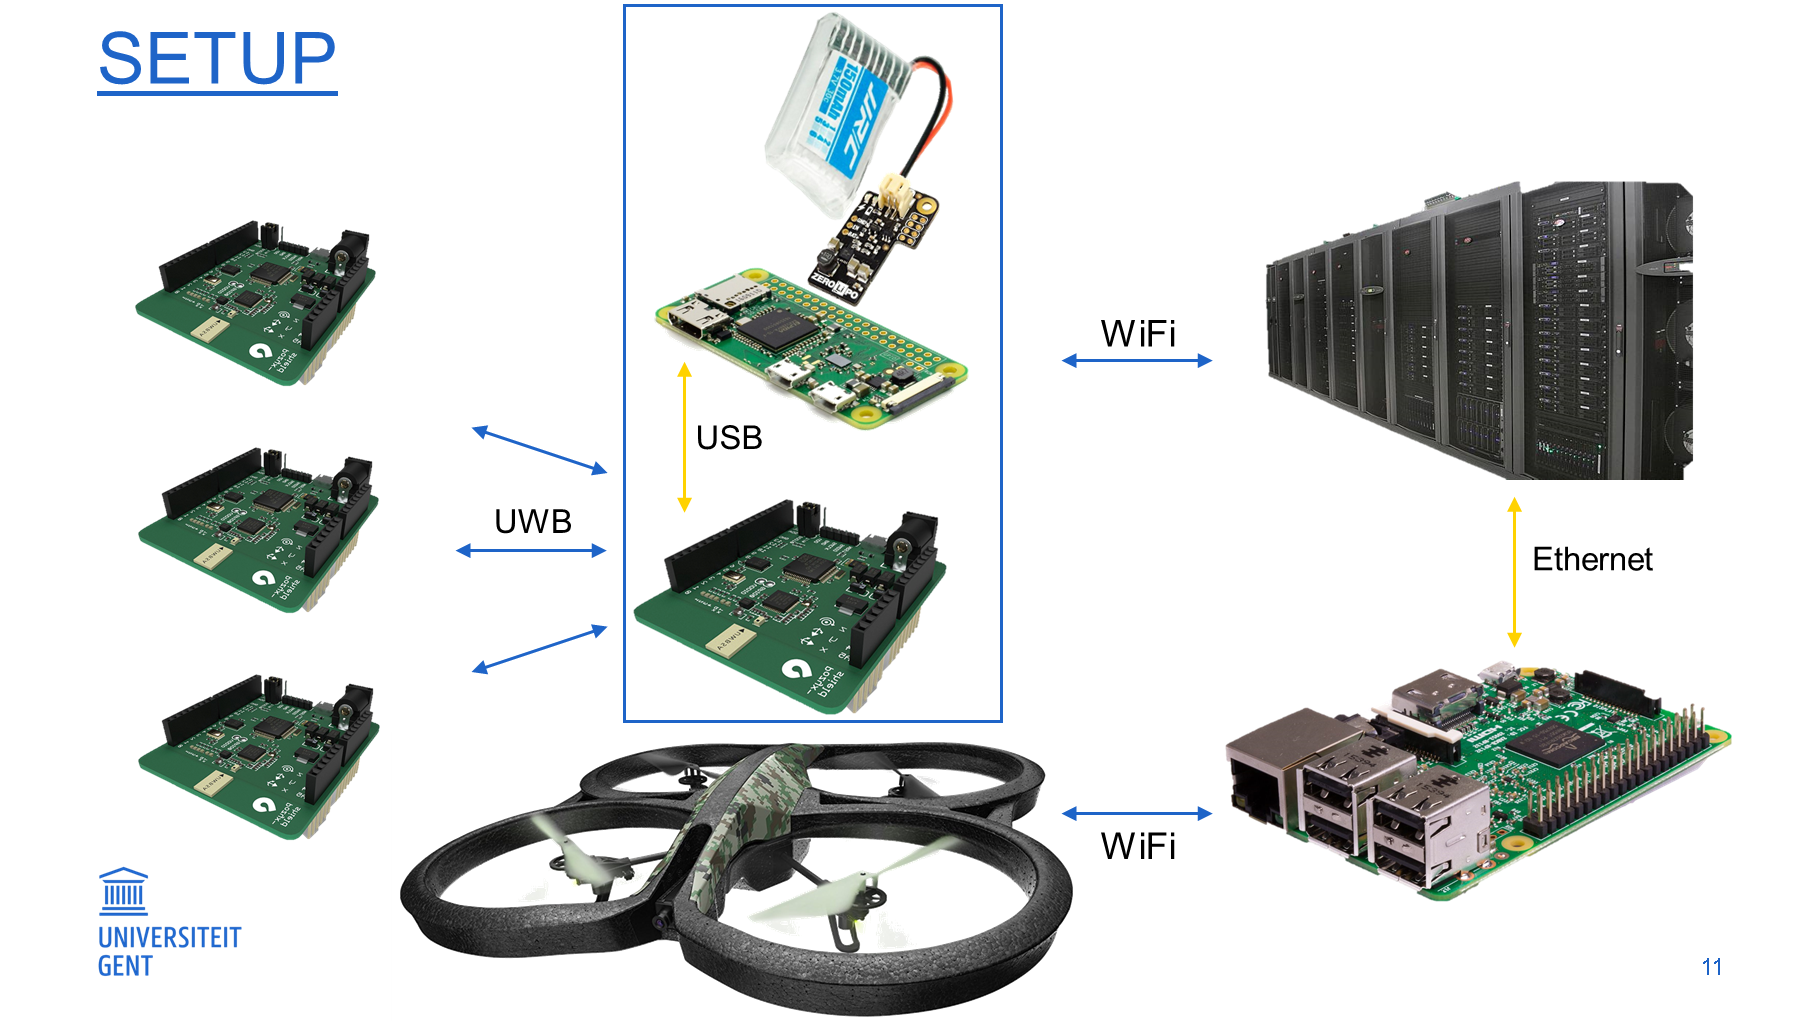
\includegraphics[width=\textwidth]{Setup_Software}
	\caption[Hardware setup, aangevuld met protocollen]{Hardware setup, aangevuld met protocollen.}
	\label{fig:setup_software}
\end{figure}

\section{Full-mesh} \label{sec:full_mesh}
